% Options for packages loaded elsewhere
\PassOptionsToPackage{unicode}{hyperref}
\PassOptionsToPackage{hyphens}{url}
%
\documentclass[
]{article}
\usepackage{amsmath,amssymb}
\usepackage{lmodern}
\usepackage{ifxetex,ifluatex}
\ifnum 0\ifxetex 1\fi\ifluatex 1\fi=0 % if pdftex
  \usepackage[T1]{fontenc}
  \usepackage[utf8]{inputenc}
  \usepackage{textcomp} % provide euro and other symbols
\else % if luatex or xetex
  \usepackage{unicode-math}
  \defaultfontfeatures{Scale=MatchLowercase}
  \defaultfontfeatures[\rmfamily]{Ligatures=TeX,Scale=1}
\fi
% Use upquote if available, for straight quotes in verbatim environments
\IfFileExists{upquote.sty}{\usepackage{upquote}}{}
\IfFileExists{microtype.sty}{% use microtype if available
  \usepackage[]{microtype}
  \UseMicrotypeSet[protrusion]{basicmath} % disable protrusion for tt fonts
}{}
\makeatletter
\@ifundefined{KOMAClassName}{% if non-KOMA class
  \IfFileExists{parskip.sty}{%
    \usepackage{parskip}
  }{% else
    \setlength{\parindent}{0pt}
    \setlength{\parskip}{6pt plus 2pt minus 1pt}}
}{% if KOMA class
  \KOMAoptions{parskip=half}}
\makeatother
\usepackage{xcolor}
\IfFileExists{xurl.sty}{\usepackage{xurl}}{} % add URL line breaks if available
\IfFileExists{bookmark.sty}{\usepackage{bookmark}}{\usepackage{hyperref}}
\hypersetup{
  pdftitle={Week 2: Introduction to R and Igraph},
  pdfauthor={Ryan Light (and jimi adams and Jim Moody and several others and Dr.~Google},
  hidelinks,
  pdfcreator={LaTeX via pandoc}}
\urlstyle{same} % disable monospaced font for URLs
\usepackage[margin=1in]{geometry}
\usepackage{color}
\usepackage{fancyvrb}
\newcommand{\VerbBar}{|}
\newcommand{\VERB}{\Verb[commandchars=\\\{\}]}
\DefineVerbatimEnvironment{Highlighting}{Verbatim}{commandchars=\\\{\}}
% Add ',fontsize=\small' for more characters per line
\usepackage{framed}
\definecolor{shadecolor}{RGB}{248,248,248}
\newenvironment{Shaded}{\begin{snugshade}}{\end{snugshade}}
\newcommand{\AlertTok}[1]{\textcolor[rgb]{0.94,0.16,0.16}{#1}}
\newcommand{\AnnotationTok}[1]{\textcolor[rgb]{0.56,0.35,0.01}{\textbf{\textit{#1}}}}
\newcommand{\AttributeTok}[1]{\textcolor[rgb]{0.77,0.63,0.00}{#1}}
\newcommand{\BaseNTok}[1]{\textcolor[rgb]{0.00,0.00,0.81}{#1}}
\newcommand{\BuiltInTok}[1]{#1}
\newcommand{\CharTok}[1]{\textcolor[rgb]{0.31,0.60,0.02}{#1}}
\newcommand{\CommentTok}[1]{\textcolor[rgb]{0.56,0.35,0.01}{\textit{#1}}}
\newcommand{\CommentVarTok}[1]{\textcolor[rgb]{0.56,0.35,0.01}{\textbf{\textit{#1}}}}
\newcommand{\ConstantTok}[1]{\textcolor[rgb]{0.00,0.00,0.00}{#1}}
\newcommand{\ControlFlowTok}[1]{\textcolor[rgb]{0.13,0.29,0.53}{\textbf{#1}}}
\newcommand{\DataTypeTok}[1]{\textcolor[rgb]{0.13,0.29,0.53}{#1}}
\newcommand{\DecValTok}[1]{\textcolor[rgb]{0.00,0.00,0.81}{#1}}
\newcommand{\DocumentationTok}[1]{\textcolor[rgb]{0.56,0.35,0.01}{\textbf{\textit{#1}}}}
\newcommand{\ErrorTok}[1]{\textcolor[rgb]{0.64,0.00,0.00}{\textbf{#1}}}
\newcommand{\ExtensionTok}[1]{#1}
\newcommand{\FloatTok}[1]{\textcolor[rgb]{0.00,0.00,0.81}{#1}}
\newcommand{\FunctionTok}[1]{\textcolor[rgb]{0.00,0.00,0.00}{#1}}
\newcommand{\ImportTok}[1]{#1}
\newcommand{\InformationTok}[1]{\textcolor[rgb]{0.56,0.35,0.01}{\textbf{\textit{#1}}}}
\newcommand{\KeywordTok}[1]{\textcolor[rgb]{0.13,0.29,0.53}{\textbf{#1}}}
\newcommand{\NormalTok}[1]{#1}
\newcommand{\OperatorTok}[1]{\textcolor[rgb]{0.81,0.36,0.00}{\textbf{#1}}}
\newcommand{\OtherTok}[1]{\textcolor[rgb]{0.56,0.35,0.01}{#1}}
\newcommand{\PreprocessorTok}[1]{\textcolor[rgb]{0.56,0.35,0.01}{\textit{#1}}}
\newcommand{\RegionMarkerTok}[1]{#1}
\newcommand{\SpecialCharTok}[1]{\textcolor[rgb]{0.00,0.00,0.00}{#1}}
\newcommand{\SpecialStringTok}[1]{\textcolor[rgb]{0.31,0.60,0.02}{#1}}
\newcommand{\StringTok}[1]{\textcolor[rgb]{0.31,0.60,0.02}{#1}}
\newcommand{\VariableTok}[1]{\textcolor[rgb]{0.00,0.00,0.00}{#1}}
\newcommand{\VerbatimStringTok}[1]{\textcolor[rgb]{0.31,0.60,0.02}{#1}}
\newcommand{\WarningTok}[1]{\textcolor[rgb]{0.56,0.35,0.01}{\textbf{\textit{#1}}}}
\usepackage{longtable,booktabs,array}
\usepackage{calc} % for calculating minipage widths
% Correct order of tables after \paragraph or \subparagraph
\usepackage{etoolbox}
\makeatletter
\patchcmd\longtable{\par}{\if@noskipsec\mbox{}\fi\par}{}{}
\makeatother
% Allow footnotes in longtable head/foot
\IfFileExists{footnotehyper.sty}{\usepackage{footnotehyper}}{\usepackage{footnote}}
\makesavenoteenv{longtable}
\usepackage{graphicx}
\makeatletter
\def\maxwidth{\ifdim\Gin@nat@width>\linewidth\linewidth\else\Gin@nat@width\fi}
\def\maxheight{\ifdim\Gin@nat@height>\textheight\textheight\else\Gin@nat@height\fi}
\makeatother
% Scale images if necessary, so that they will not overflow the page
% margins by default, and it is still possible to overwrite the defaults
% using explicit options in \includegraphics[width, height, ...]{}
\setkeys{Gin}{width=\maxwidth,height=\maxheight,keepaspectratio}
% Set default figure placement to htbp
\makeatletter
\def\fps@figure{htbp}
\makeatother
\setlength{\emergencystretch}{3em} % prevent overfull lines
\providecommand{\tightlist}{%
  \setlength{\itemsep}{0pt}\setlength{\parskip}{0pt}}
\setcounter{secnumdepth}{-\maxdimen} % remove section numbering
\ifluatex
  \usepackage{selnolig}  % disable illegal ligatures
\fi

\title{Week 2: Introduction to R and Igraph}
\author{Ryan Light (and jimi adams and Jim Moody and several others and
Dr.~Google}
\date{April 5, 2021}

\begin{document}
\maketitle

\#A few R Basics

First, lets look at some basic operators in R. This tracks nicely with
Datacamp's Introduction to R and it is recommended that you check that
out (or an equivalent) to get a hang of some of these basic operations.

\#\#Arithmetic Operators

You can use R as a caculator with arithmetic operators:

\begin{Shaded}
\begin{Highlighting}[]
\DecValTok{3}\SpecialCharTok{+}\DecValTok{4}
\end{Highlighting}
\end{Shaded}

\begin{verbatim}
## [1] 7
\end{verbatim}

You can use R to assign values (and print value):

\begin{Shaded}
\begin{Highlighting}[]
\NormalTok{a }\OtherTok{\textless{}{-}} \DecValTok{3} \SpecialCharTok{+} \DecValTok{4}
\FunctionTok{print}\NormalTok{(a)}
\end{Highlighting}
\end{Shaded}

\begin{verbatim}
## [1] 7
\end{verbatim}

\#\#Logical Operators

Logical operators can tell us whether something is true or false and is
useful for when we are working in functions.

\begin{longtable}[]{@{}ll@{}}
\toprule
Operators & Operation \\
\midrule
\endhead
== & ``is equal to'' \\
!= & ``not equal'' \\
\textless{} & ``less than'' \\
\textgreater{} & ``greater than'' \\
\textless= & ``less than or equal to'' \\
\textgreater= & ``greater than or equal to'' \\
\bottomrule
\end{longtable}

Examples

\begin{Shaded}
\begin{Highlighting}[]
\DecValTok{8} \SpecialCharTok{==} \DecValTok{8}
\end{Highlighting}
\end{Shaded}

\begin{verbatim}
## [1] TRUE
\end{verbatim}

\begin{Shaded}
\begin{Highlighting}[]
\DecValTok{8} \SpecialCharTok{!=} \DecValTok{8}
\end{Highlighting}
\end{Shaded}

\begin{verbatim}
## [1] FALSE
\end{verbatim}

\begin{Shaded}
\begin{Highlighting}[]
\ConstantTok{TRUE} \SpecialCharTok{\textgreater{}} \ConstantTok{FALSE}
\end{Highlighting}
\end{Shaded}

\begin{verbatim}
## [1] TRUE
\end{verbatim}

\begin{Shaded}
\begin{Highlighting}[]
\StringTok{"Red"} \SpecialCharTok{!=} \StringTok{"Red"}
\end{Highlighting}
\end{Shaded}

\begin{verbatim}
## [1] FALSE
\end{verbatim}

\begin{Shaded}
\begin{Highlighting}[]
\DecValTok{7} \SpecialCharTok{\textless{}=} \DecValTok{100}
\end{Highlighting}
\end{Shaded}

\begin{verbatim}
## [1] TRUE
\end{verbatim}

\begin{Shaded}
\begin{Highlighting}[]
\DecValTok{1} \SpecialCharTok{\textgreater{}=} \DecValTok{100}
\end{Highlighting}
\end{Shaded}

\begin{verbatim}
## [1] FALSE
\end{verbatim}

\#\#Functions

Functions drive much of what happens in R. Many functions operate within
packages and are ``called'' from them, but we can also make our own.

The first step is to define the function.

The basic form looks like this:

\begin{Shaded}
\begin{Highlighting}[]
\NormalTok{fake.function }\OtherTok{\textless{}{-}} \ControlFlowTok{function}\NormalTok{(vars)\{}
    \FunctionTok{print}\NormalTok{(}\StringTok{"thing to make"}\NormalTok{)}
\NormalTok{\} }
\end{Highlighting}
\end{Shaded}

And then you call the function:

\begin{Shaded}
\begin{Highlighting}[]
\FunctionTok{fake.function}\NormalTok{(}\DecValTok{1}\NormalTok{)}
\end{Highlighting}
\end{Shaded}

\begin{verbatim}
## [1] "thing to make"
\end{verbatim}

Or something better:

\begin{Shaded}
\begin{Highlighting}[]
\NormalTok{square.sum.variables }\OtherTok{\textless{}{-}} \ControlFlowTok{function}\NormalTok{(a,b)\{}
\NormalTok{  z }\OtherTok{\textless{}{-}}\NormalTok{ (a}\SpecialCharTok{+}\NormalTok{b)}\SpecialCharTok{\^{}}\DecValTok{2}
  \FunctionTok{print}\NormalTok{(z)}
\NormalTok{\} }
\FunctionTok{square.sum.variables}\NormalTok{(}\DecValTok{1}\NormalTok{,}\DecValTok{2}\NormalTok{)}
\end{Highlighting}
\end{Shaded}

\begin{verbatim}
## [1] 9
\end{verbatim}

Obviously this can get more complicated:

\begin{Shaded}
\begin{Highlighting}[]
\NormalTok{anums }\OtherTok{\textless{}{-}} \FunctionTok{c}\NormalTok{(}\DecValTok{1}\SpecialCharTok{:}\DecValTok{5}\NormalTok{) }\CommentTok{\#This is a vector}
\NormalTok{bnums }\OtherTok{\textless{}{-}} \FunctionTok{c}\NormalTok{(}\DecValTok{2}\SpecialCharTok{:}\DecValTok{6}\NormalTok{) }\CommentTok{\#This is a vector}

\FunctionTok{square.sum.variables}\NormalTok{(anums, bnums)}
\end{Highlighting}
\end{Shaded}

\begin{verbatim}
## [1]   9  25  49  81 121
\end{verbatim}

\hypertarget{object-management}{%
\subsection{Object management}\label{object-management}}

These help with your workspace. If you are using projects, these may not
be so necessary, but good to keep things cleaned up.

\begin{longtable}[]{@{}ll@{}}
\toprule
function & description \\
\midrule
\endhead
ls() & list all objects in the workspace \\
class() & returns the type of object \\
rm(e) & remove a specific object \\
ls() & list all objects in the workspace \\
rm(list=ls()) & removes all objects in workspace. \\
\bottomrule
\end{longtable}

\hypertarget{calling-help-files}{%
\subsection{Calling Help Files}\label{calling-help-files}}

Often helpful to look at help material and there are several ways to do
so. You can also google these documents which can be an easy way to
access.

\begin{longtable}[]{@{}ll@{}}
\toprule
function & description \\
\midrule
\endhead
help.start() & launch help in web browser \\
help(sqrt) & get help for specified function \\
?sqrt & same as above \\
help.search(`square root') & search help pages for topics \\
??sqrt & same as help.search() \\
\bottomrule
\end{longtable}

\#\#Objects and Object Classes Perhaps the biggest difference between R
and statistics packages is the variety of objects that R uses to store
the stuff that you make. From vectors, to matrices, dataframes, to
package-specfic objects, we will create objects as a kind of the fuel to
the function's engine.

To begin the function ``class'' helps us to identify what kind of object
we are working with. We can see this with the anums object we created
above.

\begin{Shaded}
\begin{Highlighting}[]
\FunctionTok{class}\NormalTok{(anums)}
\end{Highlighting}
\end{Shaded}

\begin{verbatim}
## [1] "integer"
\end{verbatim}

This is an integer vector. We can make vectors of other elements using
c() as we used with anums and bnums. There are a several different types
of vectors including numeric (integer is a subset of numeric) and
character vectors. R assigns a class to each vector.

\begin{Shaded}
\begin{Highlighting}[]
\CommentTok{\#Let\textquotesingle{}s make a few variables}
\NormalTok{a }\OtherTok{\textless{}{-}} \DecValTok{5}
\NormalTok{b }\OtherTok{\textless{}{-}} \DecValTok{6}
\NormalTok{c }\OtherTok{\textless{}{-}} \DecValTok{7}

\CommentTok{\# c() combines elements into a vector}
\NormalTok{e }\OtherTok{\textless{}{-}} \FunctionTok{c}\NormalTok{(a, b, c)             }

\FunctionTok{class}\NormalTok{(e)}
\end{Highlighting}
\end{Shaded}

\begin{verbatim}
## [1] "numeric"
\end{verbatim}

\begin{Shaded}
\begin{Highlighting}[]
\CommentTok{\# can also be used on character objects}

\NormalTok{f }\OtherTok{\textless{}{-}} \FunctionTok{c}\NormalTok{(}\StringTok{"This"}\NormalTok{, }\StringTok{"is"}\NormalTok{, }\StringTok{"a"}\NormalTok{, }\StringTok{"character"}\NormalTok{, }\StringTok{"vector"}\NormalTok{)    }

\CommentTok{\# And we can combine classes}
\NormalTok{g }\OtherTok{\textless{}{-}} \FunctionTok{c}\NormalTok{(e, f)                }
\FunctionTok{print}\NormalTok{(g)}
\end{Highlighting}
\end{Shaded}

\begin{verbatim}
## [1] "5"         "6"         "7"         "This"      "is"        "a"        
## [7] "character" "vector"
\end{verbatim}

\begin{Shaded}
\begin{Highlighting}[]
\FunctionTok{class}\NormalTok{(g)            }
\end{Highlighting}
\end{Shaded}

\begin{verbatim}
## [1] "character"
\end{verbatim}

We can also create vectors of sequences that are particularly helpful
when you are using functions. Again, there are several ways of creating
sequence vectors:

\begin{Shaded}
\begin{Highlighting}[]
\CommentTok{\# a sequence from 1 to 10, by 1}
\NormalTok{seq }\OtherTok{\textless{}{-}} \FunctionTok{c}\NormalTok{(}\DecValTok{1}\SpecialCharTok{:}\DecValTok{10}\NormalTok{)}

\CommentTok{\# assigning a sequence with increments !=1}
\NormalTok{seq2 }\OtherTok{\textless{}{-}} \FunctionTok{seq}\NormalTok{(}\DecValTok{2}\NormalTok{,}\DecValTok{10}\NormalTok{, }\AttributeTok{by=}\DecValTok{2}\NormalTok{)     }

\CommentTok{\# can also be reversed}
\NormalTok{seq2rev }\OtherTok{\textless{}{-}} \FunctionTok{seq}\NormalTok{(}\DecValTok{10}\NormalTok{,}\DecValTok{2}\NormalTok{, }\AttributeTok{by=}\SpecialCharTok{{-}}\DecValTok{1}\NormalTok{) }

\CommentTok{\# repeat a sequence twice}
\NormalTok{seq\_twice }\OtherTok{\textless{}{-}} \FunctionTok{rep}\NormalTok{(}\DecValTok{1}\SpecialCharTok{:}\DecValTok{5}\NormalTok{,}\AttributeTok{times=}\DecValTok{2}\NormalTok{)   }

\CommentTok{\# repeat a sequence twice, elementwise}
\NormalTok{seq\_dbl }\OtherTok{\textless{}{-}} \FunctionTok{rep}\NormalTok{(}\DecValTok{1}\SpecialCharTok{:}\DecValTok{5}\NormalTok{,}\AttributeTok{each=}\DecValTok{2}\NormalTok{)  }
\end{Highlighting}
\end{Shaded}

And we can call particular elements and use logical operators to
identify aspects of the sequences (or other vectors)

\begin{Shaded}
\begin{Highlighting}[]
\CommentTok{\# the 4th element in the assigned vector seq\_dbl}
\NormalTok{seq\_dbl[}\DecValTok{4}\NormalTok{]                  }
\end{Highlighting}
\end{Shaded}

\begin{verbatim}
## [1] 2
\end{verbatim}

\begin{Shaded}
\begin{Highlighting}[]
\CommentTok{\# the negative operator removes specified element(s) from a vector}
\NormalTok{seq[}\SpecialCharTok{{-}}\FunctionTok{c}\NormalTok{(}\DecValTok{4}\SpecialCharTok{:}\DecValTok{5}\NormalTok{)]                }
\end{Highlighting}
\end{Shaded}

\begin{verbatim}
## [1]  1  2  3  6  7  8  9 10
\end{verbatim}

\begin{Shaded}
\begin{Highlighting}[]
\CommentTok{\# is each element in seq greater tha  n 5}
\NormalTok{seq }\SpecialCharTok{\textgreater{}}\DecValTok{5}                  
\end{Highlighting}
\end{Shaded}

\begin{verbatim}
##  [1] FALSE FALSE FALSE FALSE FALSE  TRUE  TRUE  TRUE  TRUE  TRUE
\end{verbatim}

\begin{Shaded}
\begin{Highlighting}[]
\FunctionTok{any}\NormalTok{(seq}\SpecialCharTok{\textgreater{}}\DecValTok{5}\NormalTok{)                  }\CommentTok{\# are ANY elements of seq greater than 5}
\end{Highlighting}
\end{Shaded}

\begin{verbatim}
## [1] TRUE
\end{verbatim}

\begin{Shaded}
\begin{Highlighting}[]
\FunctionTok{all}\NormalTok{(seq}\SpecialCharTok{\textgreater{}}\DecValTok{5}\NormalTok{)                  }\CommentTok{\# are ALL elements of seq greater than 5}
\end{Highlighting}
\end{Shaded}

\begin{verbatim}
## [1] FALSE
\end{verbatim}

\begin{Shaded}
\begin{Highlighting}[]
\FunctionTok{which}\NormalTok{(seq}\SpecialCharTok{\textgreater{}}\DecValTok{5}\NormalTok{)                }\CommentTok{\# returns indices of elements that are TRUE}
\end{Highlighting}
\end{Shaded}

\begin{verbatim}
## [1]  6  7  8  9 10
\end{verbatim}

Another R object class is the matrix. Matrices are important in social
network analysis as many of our networks are stored as matrices. Matrix
algebra is used for constructing mixing tables (such as gender or racial
overlaps) and we also use matrix algebra for ``projecting'' two-mode
(e.g.~person-to-group networks) to one-mode networks (person-to-person
through common group membership). The matrix function makes matrices
(Note the Matrix package is also useful for constructing (and storing)
sparse matrices when you have many 0s for a network of many nodes)

\begin{Shaded}
\begin{Highlighting}[]
\NormalTok{h}\OtherTok{\textless{}{-}}\FunctionTok{matrix}\NormalTok{(}\AttributeTok{data=}\FunctionTok{c}\NormalTok{(}\DecValTok{1}\SpecialCharTok{:}\DecValTok{36}\NormalTok{), }\AttributeTok{nrow=}\DecValTok{6}\NormalTok{) }\CommentTok{\# defines a matrix, number of columns inferred, }\AlertTok{NOTE}\CommentTok{ that the default is to h               }

\NormalTok{h[}\DecValTok{4}\NormalTok{,}\DecValTok{2}\NormalTok{]                  }\CommentTok{\# returns the element in the 4th row, 2nd column}
\end{Highlighting}
\end{Shaded}

\begin{verbatim}
## [1] 10
\end{verbatim}

\begin{Shaded}
\begin{Highlighting}[]
\NormalTok{h[}\DecValTok{3}\NormalTok{,]                       }\CommentTok{\# returns the 3rd row as a vector}
\end{Highlighting}
\end{Shaded}

\begin{verbatim}
## [1]  3  9 15 21 27 33
\end{verbatim}

\begin{Shaded}
\begin{Highlighting}[]
\NormalTok{h[,}\DecValTok{3}\NormalTok{]                       }\CommentTok{\# returns the 3rd column as a vector}
\end{Highlighting}
\end{Shaded}

\begin{verbatim}
## [1] 13 14 15 16 17 18
\end{verbatim}

\begin{Shaded}
\begin{Highlighting}[]
\CommentTok{\#h[,{-}4]                 \# removes the 4th column (surpressed)}
\CommentTok{\#h[{-}2,]                 \# removes the 2nd row (surpressed)}
\NormalTok{h[}\DecValTok{3}\NormalTok{,}\DecValTok{6}\NormalTok{] }\OtherTok{\textless{}{-}} \DecValTok{0}             \CommentTok{\# replace an element}
\FunctionTok{t}\NormalTok{(h)                        }\CommentTok{\# transpose a matrix (swap rows \& columns)}
\end{Highlighting}
\end{Shaded}

\begin{verbatim}
##      [,1] [,2] [,3] [,4] [,5] [,6]
## [1,]    1    2    3    4    5    6
## [2,]    7    8    9   10   11   12
## [3,]   13   14   15   16   17   18
## [4,]   19   20   21   22   23   24
## [5,]   25   26   27   28   29   30
## [6,]   31   32    0   34   35   36
\end{verbatim}

\begin{Shaded}
\begin{Highlighting}[]
\NormalTok{h }\SpecialCharTok{\%*\%} \FunctionTok{t}\NormalTok{(h)              }\CommentTok{\# matrix multiplication (no output)}
\end{Highlighting}
\end{Shaded}

\begin{verbatim}
##      [,1] [,2] [,3] [,4] [,5] [,6]
## [1,] 2166 2262 1335 2454 2550 2646
## [2,] 2262 2364 1410 2568 2670 2772
## [3,] 1335 1410 1485 1560 1635 1710
## [4,] 2454 2568 1560 2796 2910 3024
## [5,] 2550 2670 1635 2910 3030 3150
## [6,] 2646 2772 1710 3024 3150 3276
\end{verbatim}

This brings us to data frames. Data frames are analogous to spreadsheets
or the other types of grids that comprise ``data'' in most statistical
programs. The typical data frame has rows that consist fo cases and
columns that consist of different variables. The dominance of
spreadsheets for social scientific analysis increases the appeal of
pushing things to data frames and indeed the tidy movement (see the
tidyr package) in R is in part based on the cognitive appeal of data
frame like structures.

My default is to push things into data frames when I'm in doubt.

\begin{Shaded}
\begin{Highlighting}[]
\NormalTok{i }\OtherTok{\textless{}{-}} \FunctionTok{data.frame}\NormalTok{(}\AttributeTok{age=}\DecValTok{31}\SpecialCharTok{:}\DecValTok{35}\NormalTok{, }\AttributeTok{job=}\FunctionTok{c}\NormalTok{(T,T,T,T,F),}\AttributeTok{name=}\NormalTok{LETTERS[}\DecValTok{1}\SpecialCharTok{:}\DecValTok{5}\NormalTok{])  }\CommentTok{\# assign}
\NormalTok{i[,}\DecValTok{2}\NormalTok{]                       }\CommentTok{\# works with standard matrix operators}
\end{Highlighting}
\end{Shaded}

\begin{verbatim}
## [1]  TRUE  TRUE  TRUE  TRUE FALSE
\end{verbatim}

\begin{Shaded}
\begin{Highlighting}[]
\NormalTok{i}\SpecialCharTok{$}\NormalTok{name                  }\CommentTok{\# the $ operator allows calls by labels}
\end{Highlighting}
\end{Shaded}

\begin{verbatim}
## [1] "A" "B" "C" "D" "E"
\end{verbatim}

\begin{Shaded}
\begin{Highlighting}[]
\NormalTok{i }\OtherTok{\textless{}{-}} \FunctionTok{data.frame}\NormalTok{(}\AttributeTok{age=}\DecValTok{31}\SpecialCharTok{:}\DecValTok{35}\NormalTok{, }\AttributeTok{job=}\FunctionTok{c}\NormalTok{(T,T,T,T,F),}\AttributeTok{name=}\NormalTok{LETTERS[}\DecValTok{1}\SpecialCharTok{:}\DecValTok{5}\NormalTok{], }\AttributeTok{stringsAsFactors=}\ConstantTok{FALSE}\NormalTok{)  }\CommentTok{\# getting rid of "factors"}

\NormalTok{ab\_nums }\OtherTok{\textless{}{-}} \FunctionTok{as.data.frame}\NormalTok{(}\FunctionTok{cbind}\NormalTok{(anums, bnums))}
\end{Highlighting}
\end{Shaded}

\#\#Introduction to Igraph

Igraph is a powerful network tool for visualising and analyzing social
networks. We will use igraph for many tasks in conjunction with a few
other packages specific to social network analysis (such as statnet) and
several others throughout the course.

To back up a bit, one of the cool features of R is the fact that it is
open source. Scholars can contribute R in more or less real time and,
therefore, state-of-the-art statistics are quicker to the wider
community than through expensive programs with intense gatekeeping and
less incentive to contribute.

The main way that scholars contribute to R is through the development of
packages. While base R has very powerful tools for analysis in and of
itself, R packages increase the power of R exponentially and in many
ways make R easier to use.

Each package needs to be installed into R prior to use. Note: You can
comment out code with \#. I do that here to prevent running the install.

\begin{Shaded}
\begin{Highlighting}[]
\CommentTok{\#install.packages(igraph)}
\end{Highlighting}
\end{Shaded}

You only need to do this once if there are no updates. When you update R
to the latest version, you should be sure to check for package updates.

\begin{Shaded}
\begin{Highlighting}[]
\CommentTok{\#update.packages("igraph")}
\end{Highlighting}
\end{Shaded}

Again, you don't have to do this every time you use R or want ot use
igraph.

\emph{You} do have to load packages outside of base R into each session
that you begin.

\begin{Shaded}
\begin{Highlighting}[]
\FunctionTok{library}\NormalTok{(igraph)}
\end{Highlighting}
\end{Shaded}

\begin{verbatim}
## 
## Attaching package: 'igraph'
\end{verbatim}

\begin{verbatim}
## The following objects are masked from 'package:stats':
## 
##     decompose, spectrum
\end{verbatim}

\begin{verbatim}
## The following object is masked from 'package:base':
## 
##     union
\end{verbatim}

\#\#\#Bringing Data Into igraph

There are many different ways to bring data into igraph. Remember that
the two main ways to store network data is either an edge list (two
columns: one sender, one receiver) or an adjacency matrix (i rows and j
columns are the same people and the cells indicate a connection between
the i row and j column). If you can make an edgelist or a matrix you can
load the data into igraph.

\#\#\#Bringing Data Into igraph: importing csv Files

First, we can bring in the data into r using the base function
read.csv(). The first example is an undirected toy network. Note that we
will keep the column names as indicated by ``header=T''

\begin{Shaded}
\begin{Highlighting}[]
\NormalTok{toy.undirected }\OtherTok{\textless{}{-}} \FunctionTok{read.csv}\NormalTok{(}\StringTok{"data/simple\_undirected.csv"}\NormalTok{, }\AttributeTok{header=}\NormalTok{T)   }\CommentTok{\# reading in the undirected mixing example}

\FunctionTok{print}\NormalTok{(toy.undirected)}
\end{Highlighting}
\end{Shaded}

\begin{verbatim}
##   id alt1 alt2 alt3 attr1
## 1  1    3   NA   NA     1
## 2  2    3   NA   NA     1
## 3  3    1    2    4     1
## 4  4    3    5    6     0
## 5  5    4    6   NA     0
## 6  6    4    5   NA     0
\end{verbatim}

Now we need to clean the data up a bit to make an edge list. If we look
above, we can see another way of storing network data - the adjacency
list. Adjacency lists consist of nodes and the alters that are adjacent
to them. So person 6 is connected to alters 4 and 5. We first separate
the adjacency list and the nodal attribute. We can use the row()
function to transform the adjacency list into a edge list.

\begin{Shaded}
\begin{Highlighting}[]
\NormalTok{ties}\OtherTok{\textless{}{-}} \FunctionTok{subset}\NormalTok{(toy.undirected,}\AttributeTok{select=}\FunctionTok{c}\NormalTok{(alt1,alt2,alt3))  }\CommentTok{\# stripping off just the adjacency list}
\NormalTok{nodes }\OtherTok{\textless{}{-}} \FunctionTok{subset}\NormalTok{(toy.undirected,}\AttributeTok{select=}\FunctionTok{c}\NormalTok{(id,attr1))      }\CommentTok{\# stripping off just the attributes}
\NormalTok{toy.df }\OtherTok{\textless{}{-}} \FunctionTok{data.frame}\NormalTok{(}\AttributeTok{snd =} \FunctionTok{row}\NormalTok{(ties)[}\SpecialCharTok{!}\FunctionTok{is.na}\NormalTok{(ties)], }\AttributeTok{rcv =}\NormalTok{ ties[}\SpecialCharTok{!}\FunctionTok{is.na}\NormalTok{(ties)])   }
\end{Highlighting}
\end{Shaded}

Igraph requires that we make an igraph object and there are several ways
of doing so. In this example, we use graph.data.frame() to make this
object. We indicate that the network is undirected and point igraph to
the nodes data frame for information on nodal attributes.

\begin{Shaded}
\begin{Highlighting}[]
\NormalTok{toy.g }\OtherTok{\textless{}{-}} \FunctionTok{graph.data.frame}\NormalTok{(toy.df, }\AttributeTok{directed=}\NormalTok{F, }\AttributeTok{vertices=}\NormalTok{nodes)   }\CommentTok{\# converting to an igraph “graph” object}
\end{Highlighting}
\end{Shaded}

We can use plot.igraph() function to visualize the graph. We use the
attribute that was introduced from nodes to color the nodes (Be sure
it's the same, *2 is to avoid using the same color for the label/node
color).

\begin{Shaded}
\begin{Highlighting}[]
\FunctionTok{plot.igraph}\NormalTok{(toy.g, }\AttributeTok{vertex.color=}\FunctionTok{V}\NormalTok{(toy.g)}\SpecialCharTok{$}\NormalTok{attr1}\SpecialCharTok{*}\DecValTok{2}\NormalTok{)   }
\end{Highlighting}
\end{Shaded}

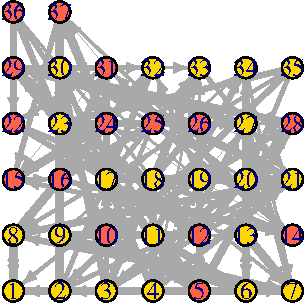
\includegraphics{week2_introduction_to_r2_files/figure-latex/unnamed-chunk-20-1.pdf}

The above toy graph consisted of undirected ties. Some graphs have
directed ties. Let's check out how igraph plots these.

Note we can also use the graph\_from\_adj\_list function to bring
adjacency lists into igraph. If you want an undirected graph, then
mode=``all''. And if you want a directed graph of sent ties, then
mode=``out''.

\begin{Shaded}
\begin{Highlighting}[]
\NormalTok{toy.directed }\OtherTok{\textless{}{-}} \FunctionTok{read.csv}\NormalTok{(}\StringTok{"data/simple\_directed.csv"}\NormalTok{, }\AttributeTok{header=}\NormalTok{T)  }
\NormalTok{nodes }\OtherTok{\textless{}{-}} \FunctionTok{subset}\NormalTok{(toy.directed,}\AttributeTok{select=}\FunctionTok{c}\NormalTok{(id,attr1))        }
\NormalTok{ties }\OtherTok{\textless{}{-}} \FunctionTok{subset}\NormalTok{(toy.directed,}\AttributeTok{select=}\FunctionTok{c}\NormalTok{(alt1,alt2,alt3))   }

\NormalTok{ties[}\FunctionTok{is.na}\NormalTok{(ties)] }\OtherTok{\textless{}{-}} \DecValTok{0}

\NormalTok{toy.g.directed }\OtherTok{\textless{}{-}} \FunctionTok{graph\_from\_adj\_list}\NormalTok{(ties}\SpecialCharTok{+}\DecValTok{1}\NormalTok{, }\AttributeTok{mode=}\StringTok{"out"}\NormalTok{)}
\end{Highlighting}
\end{Shaded}

You can store attributes as follows (make sure the order is the same)

\begin{Shaded}
\begin{Highlighting}[]
\FunctionTok{V}\NormalTok{(toy.g.directed)}\SpecialCharTok{$}\NormalTok{attribute }\OtherTok{\textless{}{-}}\NormalTok{ nodes}\SpecialCharTok{$}\NormalTok{attr1}
\end{Highlighting}
\end{Shaded}

\begin{verbatim}
## Warning in vattrs[[name]][index] <- value: number of items to replace is not a
## multiple of replacement length
\end{verbatim}

And plot the directed graph

\begin{Shaded}
\begin{Highlighting}[]
\FunctionTok{plot.igraph}\NormalTok{(}\FunctionTok{simplify}\NormalTok{(toy.g.directed), }\AttributeTok{vertex.color=}\FunctionTok{V}\NormalTok{(toy.g.directed)}\SpecialCharTok{$}\NormalTok{attribute}\SpecialCharTok{*}\DecValTok{2}\NormalTok{)}
\end{Highlighting}
\end{Shaded}

\includegraphics{week2_introduction_to_r2_files/figure-latex/unnamed-chunk-23-1.pdf}

\begin{Shaded}
\begin{Highlighting}[]
\FunctionTok{V}\NormalTok{(toy.g.directed)         }\CommentTok{\# lists the specified vertices}
\end{Highlighting}
\end{Shaded}

\begin{verbatim}
## + 7/7 vertices, from ecdeb07:
## [1] 1 2 3 4 5 6 7
\end{verbatim}

\begin{Shaded}
\begin{Highlighting}[]
\FunctionTok{E}\NormalTok{(toy.g.directed)                   }\CommentTok{\# gives the edgelist of the specified graph}
\end{Highlighting}
\end{Shaded}

\begin{verbatim}
## + 18/18 edges from ecdeb07:
##  [1] 1->4 1->3 1->4 1->7 1->6 1->1 2->1 2->1 2->5 2->6 2->1 2->1 3->1 3->1 3->1
## [16] 3->7 3->1 3->1
\end{verbatim}

\#\#\#Bringing Data into igraph: edge lists

You can also write edge lists directly into igraph. Igraph will read
each pair as an edge. Here we have indicated an undirected graph by
directed=F.

\begin{Shaded}
\begin{Highlighting}[]
\NormalTok{edge.list }\OtherTok{\textless{}{-}} \FunctionTok{c}\NormalTok{(}\DecValTok{1}\NormalTok{,}\DecValTok{3}\NormalTok{, }\DecValTok{2}\NormalTok{,}\DecValTok{3}\NormalTok{, }\DecValTok{3}\NormalTok{,}\DecValTok{4}\NormalTok{, }\DecValTok{4}\NormalTok{,}\DecValTok{5}\NormalTok{, }\DecValTok{4}\NormalTok{,}\DecValTok{6}\NormalTok{, }\DecValTok{5}\NormalTok{,}\DecValTok{6}\NormalTok{)}

\NormalTok{exa\_g }\OtherTok{\textless{}{-}} \FunctionTok{graph}\NormalTok{(edge.list, }\AttributeTok{directed=}\NormalTok{F)   }
\FunctionTok{V}\NormalTok{(exa\_g)}\SpecialCharTok{$}\NormalTok{attr1 }\OtherTok{\textless{}{-}} \FunctionTok{c}\NormalTok{(}\DecValTok{1}\NormalTok{,}\DecValTok{1}\NormalTok{,}\DecValTok{1}\NormalTok{,}\DecValTok{0}\NormalTok{,}\DecValTok{0}\NormalTok{,}\DecValTok{0}\NormalTok{)        }\CommentTok{\# attach the attribute vector}
\FunctionTok{plot.igraph}\NormalTok{(exa\_g, }\AttributeTok{vertex.color=}\FunctionTok{V}\NormalTok{(exa\_g)}\SpecialCharTok{$}\NormalTok{attr1}\SpecialCharTok{*}\DecValTok{2}\NormalTok{)   }\CommentTok{\# how’s it look?}
\end{Highlighting}
\end{Shaded}

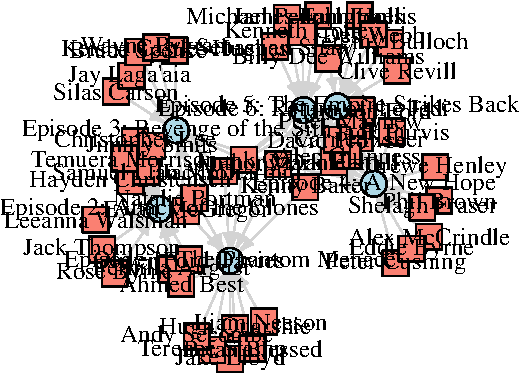
\includegraphics{week2_introduction_to_r2_files/figure-latex/unnamed-chunk-24-1.pdf}

\#\#\#Bringing Data into igraph: read.graph

We can also bring data into igraph via other programs like the networks
program Pajek. Pajek is a popular program used to visualize and analyze
social networks. The file extensions for Pajek include .net for the
network file and .clu for attributes which are often kept in separate
files.

read.graph() function will read networks from other programs. format=
identifies the type of file (e.g.~the program in which the file was
generated)

This Valente data captures the friendship ties in a fifth grade
classroom.

\begin{Shaded}
\begin{Highlighting}[]
\NormalTok{valente }\OtherTok{\textless{}{-}} \FunctionTok{read.graph}\NormalTok{(}\StringTok{"data/valente.net"}\NormalTok{, }\AttributeTok{format=}\StringTok{"pajek"}\NormalTok{)   }\CommentTok{\# getting the adjacency matrix}
\end{Highlighting}
\end{Shaded}

Next, we bring the gender attribute (valente.clu) file from pajek into
R. We skip the first line (skip=1) because pajek files include one
additional line that is not needed.

\begin{Shaded}
\begin{Highlighting}[]
\NormalTok{valente }\OtherTok{\textless{}{-}} \FunctionTok{read.graph}\NormalTok{(}\StringTok{"data/valente.net"}\NormalTok{, }\AttributeTok{format=}\StringTok{"pajek"}\NormalTok{)   }
\NormalTok{gender }\OtherTok{\textless{}{-}} \FunctionTok{as.matrix}\NormalTok{(}\FunctionTok{read.table}\NormalTok{(}\StringTok{"data/valente.clu"}\NormalTok{, }\AttributeTok{skip=}\DecValTok{1}\NormalTok{))}

\FunctionTok{V}\NormalTok{(valente)}\SpecialCharTok{$}\NormalTok{gender }\OtherTok{\textless{}{-}} \FunctionTok{as.vector}\NormalTok{(gender)              }\CommentTok{\# attaching the attribute, make numeric}
\end{Highlighting}
\end{Shaded}

Let's look at the graph. What can we learn about this classroom given
the friendship nominations? Note the attribute key: blue=girls and
white=boys

\begin{Shaded}
\begin{Highlighting}[]
\FunctionTok{plot.igraph}\NormalTok{(valente, }\AttributeTok{vertex.color=}\FunctionTok{V}\NormalTok{(valente)}\SpecialCharTok{$}\NormalTok{gender}\SpecialCharTok{*}\DecValTok{2}\NormalTok{, }\AttributeTok{layout=}\NormalTok{layout.fruchterman.reingold)  }
\end{Highlighting}
\end{Shaded}

\includegraphics{week2_introduction_to_r2_files/figure-latex/unnamed-chunk-27-1.pdf}

\#\#\#Bringing Data into igraph: two-mode data

In a few weeks we will talk about duality and two-mode networks. Here is
a quick example of how we might bring a two-mode network into igraph.

I've collected data on Star Wars movies from imdb.com. I copied and
pasted the top 15 actors in each of the first six movies into excel and
saved as a csv.

\begin{Shaded}
\begin{Highlighting}[]
\NormalTok{star.wars }\OtherTok{\textless{}{-}} \FunctionTok{read.csv}\NormalTok{(}\StringTok{"data/star\_wars.csv"}\NormalTok{ , }\AttributeTok{header=}\ConstantTok{TRUE}\NormalTok{)}

\NormalTok{sw.g }\OtherTok{\textless{}{-}} \FunctionTok{graph.data.frame}\NormalTok{(star.wars)}

\FunctionTok{print}\NormalTok{(sw.g)}
\end{Highlighting}
\end{Shaded}

\begin{verbatim}
## IGRAPH fdab43e DN-- 56 90 -- 
## + attr: name (v/c)
## + edges from fdab43e (vertex names):
##  [1] Liam Neeson       ->Episode 1: The Phantom Menace
##  [2] Ewan McGregor     ->Episode 1: The Phantom Menace
##  [3] Natalie Portman   ->Episode 1: The Phantom Menace
##  [4] Jake Lloyd        ->Episode 1: The Phantom Menace
##  [5] Ian McDiarmid     ->Episode 1: The Phantom Menace
##  [6] Pernilla August   ->Episode 1: The Phantom Menace
##  [7] Oliver Ford Davies->Episode 1: The Phantom Menace
##  [8] Hugh Quarshie     ->Episode 1: The Phantom Menace
## + ... omitted several edges
\end{verbatim}

\begin{Shaded}
\begin{Highlighting}[]
\FunctionTok{bipartite.mapping}\NormalTok{(sw.g)}
\end{Highlighting}
\end{Shaded}

\begin{verbatim}
## $res
## [1] TRUE
## 
## $type
##  [1] FALSE FALSE FALSE FALSE FALSE FALSE FALSE FALSE FALSE FALSE FALSE FALSE
## [13] FALSE FALSE FALSE FALSE FALSE FALSE FALSE FALSE FALSE FALSE FALSE FALSE
## [25] FALSE FALSE FALSE FALSE FALSE FALSE FALSE FALSE FALSE FALSE FALSE FALSE
## [37] FALSE FALSE FALSE FALSE FALSE FALSE FALSE FALSE FALSE FALSE FALSE FALSE
## [49] FALSE FALSE  TRUE  TRUE  TRUE  TRUE  TRUE  TRUE
\end{verbatim}

\begin{Shaded}
\begin{Highlighting}[]
\FunctionTok{V}\NormalTok{(sw.g)}\SpecialCharTok{$}\NormalTok{type }\OtherTok{\textless{}{-}} \FunctionTok{bipartite.mapping}\NormalTok{(sw.g)}\SpecialCharTok{$}\NormalTok{type}

\FunctionTok{V}\NormalTok{(sw.g)}\SpecialCharTok{$}\NormalTok{color }\OtherTok{\textless{}{-}} \FunctionTok{ifelse}\NormalTok{(}\FunctionTok{V}\NormalTok{(sw.g)}\SpecialCharTok{$}\NormalTok{type, }\StringTok{"lightblue"}\NormalTok{, }\StringTok{"salmon"}\NormalTok{)}
\FunctionTok{V}\NormalTok{(sw.g)}\SpecialCharTok{$}\NormalTok{shape }\OtherTok{\textless{}{-}} \FunctionTok{ifelse}\NormalTok{(}\FunctionTok{V}\NormalTok{(sw.g)}\SpecialCharTok{$}\NormalTok{type, }\StringTok{"circle"}\NormalTok{, }\StringTok{"square"}\NormalTok{)}
\FunctionTok{E}\NormalTok{(sw.g)}\SpecialCharTok{$}\NormalTok{color }\OtherTok{\textless{}{-}} \StringTok{"lightgray"}

\FunctionTok{plot.igraph}\NormalTok{(sw.g, }\AttributeTok{layout=}\NormalTok{layout.fruchterman.reingold, }\AttributeTok{vertex.label.color=}\StringTok{"black"}\NormalTok{, }\AttributeTok{edge.arrow.size=}\NormalTok{.}\DecValTok{5}\NormalTok{)}
\end{Highlighting}
\end{Shaded}

\includegraphics{week2_introduction_to_r2_files/figure-latex/unnamed-chunk-28-1.pdf}
How to read the Igraph code:

``The first line always starts with IGRAPH, showing you that the object
is an igraph graph. Then a four letter long code string is printed. The
first letter distinguishes between directed (`D') and undirected (`U')
graphs. The second letter is `N' for named graphs, i.e.~graphs with the
name vertex attribute set. The third letter is `W' for weighted graphs,
i.e.~graphs with the weight edge attribute set. The fourth letter is `B'
for bipartite graphs, i.e.~for graphs with the type vertex attribute
set.'' (from \url{http://igraph.org/r/doc/print.igraph.html})

\#\#\#Family Tree Example

The first family tree has just one step and one tie type

\begin{Shaded}
\begin{Highlighting}[]
\NormalTok{fam.edge.list }\OtherTok{\textless{}{-}} \FunctionTok{c}\NormalTok{(}\StringTok{"Ryan"}\NormalTok{,}\StringTok{"Henry"}\NormalTok{,  }\StringTok{"Mike"}\NormalTok{,}\StringTok{"Ryan"}\NormalTok{,  }\StringTok{"Linda"}\NormalTok{,}\StringTok{"Ryan"}\NormalTok{)}
\NormalTok{fam\_g }\OtherTok{\textless{}{-}} \FunctionTok{graph}\NormalTok{(fam.edge.list, }\AttributeTok{directed=}\NormalTok{T)   }
\NormalTok{fam\_g}\SpecialCharTok{$}\NormalTok{label }\OtherTok{=} \FunctionTok{names}\NormalTok{(}\FunctionTok{c}\NormalTok{(}\StringTok{"1"} \OtherTok{=} \StringTok{"Henry"}\NormalTok{, }\StringTok{"2"}\OtherTok{=}\StringTok{"Ryan"}\NormalTok{, }\StringTok{"3"}\OtherTok{=}\StringTok{"Mike"}\NormalTok{, }\StringTok{"4"}\OtherTok{=}\StringTok{"Linda"}\NormalTok{))}

\FunctionTok{plot.igraph}\NormalTok{(fam\_g)}\CommentTok{\# how’s it look?}
\end{Highlighting}
\end{Shaded}

\includegraphics{week2_introduction_to_r2_files/figure-latex/unnamed-chunk-29-1.pdf}

\end{document}
